\documentclass[10pt]{article}
\usepackage{amsmath,amsfonts,times}
\usepackage{graphicx,color,tikz}
\usepackage[paperwidth=17.6cm,paperheight=10.3cm,lmargin=0in,rmargin=0in,tmargin=0.in,bmargin=0.in]{geometry}
\usepackage{bm}
\usetikzlibrary{arrows.meta,calc,positioning}

% The march of a ray toward a surface: sphere tracing where the value is a distance (top), fixed steps and
% bisection where it is not (bottom). The scene on top is a floor with a round bump; every circle is drawn
% with the true distance from its center to that surface, so each one touches the surface.
\definecolor{cray}{rgb}{0.10,0.35,0.80}
\definecolor{cband}{rgb}{0.95,0.60,0.10}
\definecolor{chit}{rgb}{0.80,0.10,0.10}
\definecolor{csolid}{rgb}{0.78,0.78,0.80}

\tikzset{
  ray/.style={-{Stealth[length=2.5mm]}, line width=1.1pt, draw=cray},
  stepcircle/.style={draw=cray!70, thin},
  sample/.style={circle, fill=cray, inner sep=0pt, minimum width=3.2pt},
  hit/.style={circle, fill=chit, draw=white, inner sep=0pt, minimum width=5pt},
  note/.style={font=\scriptsize, align=left, fill=white, fill opacity=0.85, text opacity=1, inner sep=2pt},
}

% The surface: a floor at y = -1.8 with a half-disc bump of radius 1.6 at x = 8. The tolerance (0.15 here,
% drawn far wider than the default) is a band on either side of it.
\newcommand{\surface}{(-0.5,-1.8) -- (6.4,-1.8) arc[start angle=180, end angle=0, radius=1.6] -- (10.6,-1.8)}
\newcommand{\scene}{%
  \draw[cband, opacity=0.45, line width=2.16mm] \surface;
  \fill[csolid] \surface -- (10.6,-2.5) -- (-0.5,-2.5) -- cycle;
  \draw[thick, black!70] \surface;
}

\begin{document}
\nopagecolor
\centering
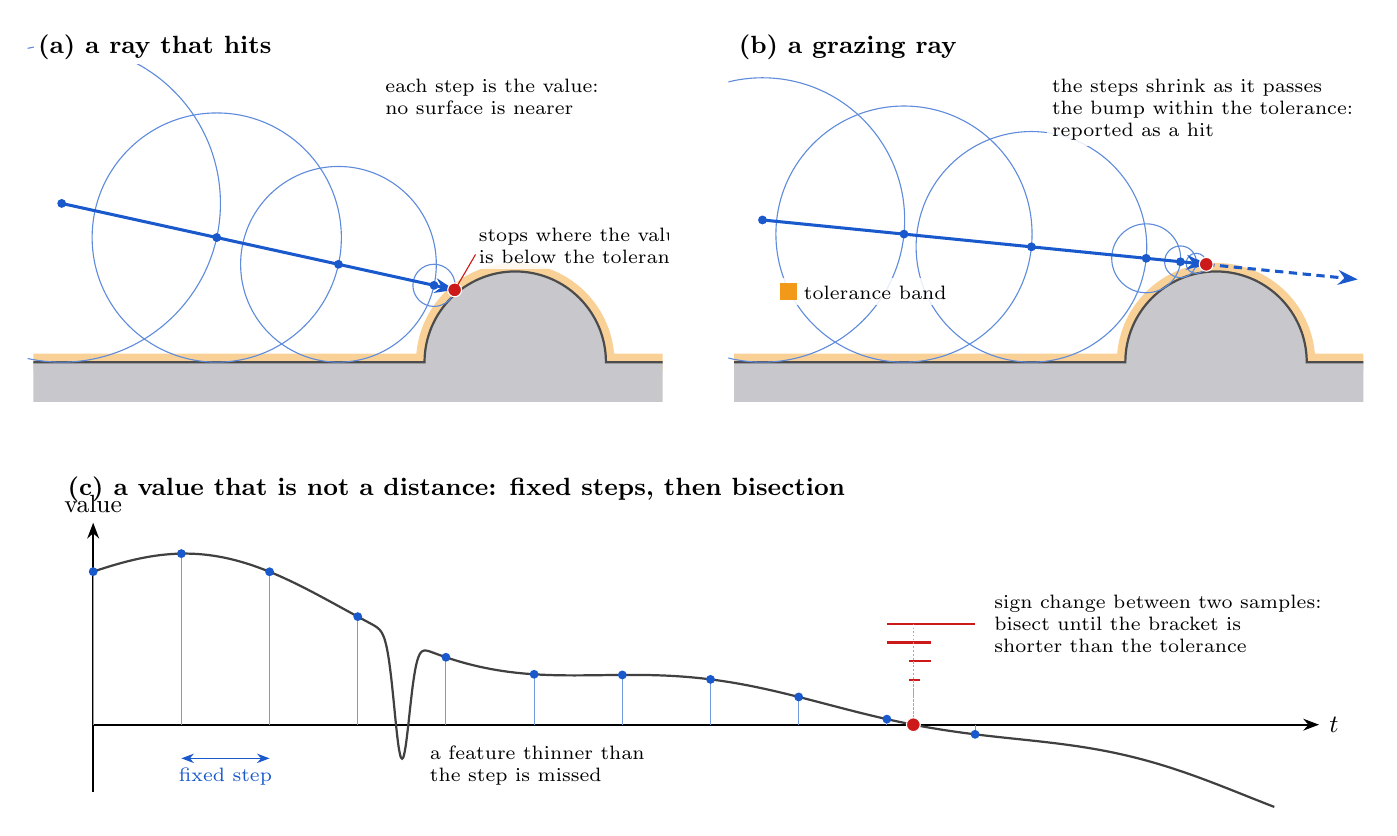
\begin{tikzpicture}[x=1cm, y=1cm]

  % ── (a) A ray that hits: the steps shrink as it nears the surface, and the march stops inside the band.
  \begin{scope}[scale=0.72]
    \clip (-0.6,-2.6) rectangle (10.7,4.1);
    \scene
    \draw[stepcircle] (0.000, 1.000) circle (2.800);
    \draw[stepcircle] (2.735, 0.398) circle (2.198);
    \draw[stepcircle] (4.882,-0.074) circle (1.726);
    \draw[stepcircle] (6.567,-0.445) circle (0.372);
    \draw[ray] (0,1.0) -- (6.931,-0.525);
    \foreach \p in {(0.000,1.000), (2.735,0.398), (4.882,-0.074), (6.567,-0.445)} {
      \node[sample] at \p {};
    }
    \node[hit] at (6.931,-0.525) {};
    \node[font=\small\bfseries, anchor=north west, fill=white, inner sep=1.5pt] at (-0.5,4.05) {(a) a ray that hits};
    \node[note, anchor=north west] at (5.6,3.3) {each step is the value:\\no surface is nearer};
    \node[note, anchor=west] at (7.25,0.25) {stops where the value\\is below the tolerance};
    \draw[chit, thin] (7.3,0.1) -- (6.98,-0.45);
  \end{scope}

  % ── (b) A grazing ray: it passes the bump within the tolerance, never crossing, and counts as a hit.
  \begin{scope}[shift={(8.9,0)}, scale=0.72]
    \clip (-0.6,-2.6) rectangle (10.7,4.1);
    \scene
    \draw[stepcircle] (0.000, 0.708) circle (2.508);
    \draw[stepcircle] (2.496, 0.459) circle (2.259);
    \draw[stepcircle] (4.744, 0.234) circle (2.034);
    \draw[stepcircle] (6.768, 0.032) circle (0.608);
    \draw[stepcircle] (7.372,-0.029) circle (0.279);
    \draw[stepcircle] (7.650,-0.057) circle (0.178);
    \draw[cray, line width=1.1pt, densely dashed, -{Stealth[length=2.5mm]}] (7.827,-0.074) -- (10.5,-0.34);
    \draw[ray] (0,0.708) -- (7.827,-0.074);
    \foreach \p in {(0.000,0.708), (2.496,0.459), (4.744,0.234), (6.768,0.032), (7.372,-0.029), (7.650,-0.057)} {
      \node[sample] at \p {};
    }
    \node[hit] at (7.827,-0.074) {};
    \node[font=\small\bfseries, anchor=north west, fill=white, inner sep=1.5pt] at (-0.5,4.05) {(b) a grazing ray};
    \node[note, anchor=north west] at (5.0,3.3) {the steps shrink as it passes\\the bump within the tolerance:\\reported as a hit};
    \node[note, anchor=north west] at (0.2,-0.3) {\textcolor{cband}{\rule{6pt}{6pt}}~tolerance band};
  \end{scope}

  % ── (c) A value that is not a distance, along the ray: fixed steps, and bisection at a sign change.
  \begin{scope}[shift={(0.4,-5.9)}, x=1.12cm, y=0.95cm]
    \node[font=\small\bfseries, anchor=north west] at (-0.4,3.45) {(c) a value that is not a distance: fixed steps, then bisection};
    \draw[-{Stealth[length=2mm]}, thick] (0,0) -- (13.9,0) node[right, font=\small] {$t$};
    \draw[-{Stealth[length=2mm]}, thick] (0,-0.9) -- (0,2.7) node[above, font=\small] {value};
    \draw[black!75, thick, domain=0:13.4, samples=500, smooth]
      plot (\x, {0.22*(9.3-\x)*(1+0.3*sin(\x r)) - 1.6*exp(-((\x-3.5)/0.12)^2)});
    \foreach \t in {0,...,10} {
      \pgfmathsetmacro{\v}{0.22*(9.3-\t)*(1+0.3*sin(\t r)) - 1.6*exp(-((\t-3.5)/0.12)^2)}
      \draw[cray!60] (\t,0) -- (\t,\v);
      \node[sample] at (\t,\v) {};
    }
    % The step, and the thin feature between two samples.
    \draw[{Stealth[length=1.6mm]}-{Stealth[length=1.6mm]}, cray] (1,-0.45) -- node[below, font=\scriptsize] {fixed step} (2,-0.45);
    \node[note, anchor=west] at (3.75,-0.55) {a feature thinner than\\the step is missed};
    % The sign change between samples 9 and 10, and the bisection that narrows it.
    \draw[chit, thick] (9,1.35) -- (10,1.35);
    \draw[chit, thick] (9,1.10) -- (9.5,1.10);
    \draw[chit, thick] (9.25,0.85) -- (9.5,0.85);
    \draw[chit, thick] (9.25,0.60) -- (9.375,0.60);
    \foreach \y in {1.35,1.10,0.85,0.60} { \draw[chit!50, densely dotted] (9.3,\y) -- (9.3,0); }
    \node[hit] at (9.3,0) {};
    \node[note, anchor=west] at (10.15,1.35) {sign change between two samples:\\bisect until the bracket is\\shorter than the tolerance};
  \end{scope}

\end{tikzpicture}

\end{document}
